\section{Sketch Construction}
\label{sec:sketch}
Our \emph{Sketch} data structure is a multidimensional, graph-based model of incoming data streams. Each resource in the system maintains an in-memory Sketch instance that can be queried to retrieve statistical properties about the underlying data or discover how features interact. Due to the magnitude of inbound data volumes, storing each individual record in main memory is not practical. Therefore, the queries supported by our framework are facilitated by compact, online metadata collection and quantization methods. These techniques ensure high accuracy while also conforming to the memory requirements of the system. To further improve accuracy, we bias our algorithms toward the most recent data points while reducing the resolution of the oldest.

\subsection{Graph Structure}
Sketch instances are maintained as hierarchical graphs with feature values stored in the vertices. Each \emph{plane} in the graph represents a particular \emph{feature type}, and traversing through vertices in this feature hierarchy reduces the search space of a query. Paths taken through the graph during a lookup operation are influenced by the specificity of the query, with additional feature expressions constraining the \emph{query scope}. Figure~\ref{fig:sketch} demonstrates the structure of a Sketch and highlights a query and its scope. Note that vertices on the same plane are connected to allow range queries, and that any subset of the graph can be retrieved and manipulated in the same fashion as the overall Sketch.

\begin{figure}
    \centerline{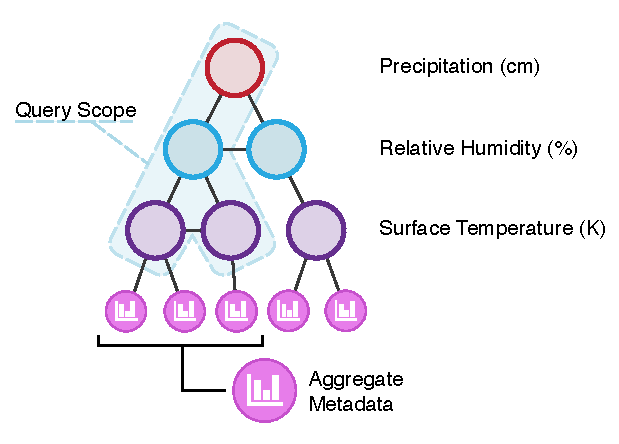
\includegraphics[width=3.5in]{figures/sketch.pdf}}
    \caption{A simplified Sketch instance with a three-plane hierarchy and sample query scope, leading to several metadata leaves. In production settings, Sketches contain hundreds of thousands of vertices and edges.}
    \label{fig:sketch}
\end{figure}

Metadata records for paths through the feature hierarchy are stored at leaf nodes. Each record contains a variety of statistics that are updated in an online fashion using Welford's~Algorithm~\cite{welford1962note}. This includes cross-feature relationships, such as the correlation between temperature values and humidity or the reflectivity of the earth and cloud cover. Leaf nodes may be \emph{merged} to combine their respective summary statistics into a single aggregate summary. This allows queries to be evaluated across multiple Sketches on disparate resources and then merged into a single, coherent result Sketch.

The number of unique feature types stored in the graph directly influences the size of the hierarchy, impacting memory consumption. However, the number of vertices and edges that must be maintained by a graph can be managed by manipulating the hierarchical configuration. For instance, the memory impact of features that exhibit high variance over a large range can be mitigated by placing them toward the top of the hierarchy, while boolean features or those with a low variety of possible values should be situated toward the bottom of the graph. Most importantly, leaf vertices must contain the spatial locations of the records to facilitate our scaling strategy; storing this information at the top of the hierarchy would simply result in an individual Sketch being maintained for each spatial location, eliminating the memory consumption benefits of the data structure. Feature planes are reconfigured dynamically based on their corresponding vertex \emph{fan-out} during the initial population of the graph. In this phase full-resolution feature values are stored at each vertex, but once a steady state is reached the \emph{quantization} process begins.

\subsection{Density-Driven Quantization}
Maintaining data points, statistics, and cross-feature relationships in memory at full resolution is infeasible when faced with voluminous datasets, even when load is balanced over several computing resources. To reduce the memory consumption of Sketch instances we perform \emph{quantization} --- targeted reduction of resolution --- which allows vertices in the graph to be merged, thus enabling single vertices to represent a collection of values. We determine which vertices should be merged by splitting each range of feature values into a configurable number of \emph{bins}. After quantization, each vertex represents a collection of observations over a range of values.

To determine the size and quantity of these bins, Sketches maintain additional graph metadata provided by the multivariate online kernel density estimation (oKDE) algorithm developed by Kristan et al. \cite{kristan2011multivariate}. oKDE assimilates data incrementally at runtime to create a dynamic probability density function (PDF) for each feature type. The smoothing parameter used to create the PDF, called the \emph{bandwidth}, is selected autonomously using Silverman's~rule~\cite{silverman1986density}. During the quantization process, these PDFs are used to ensure that each bin is assigned an approximately equal proportion of the feature density, while the overall number of bins is influenced by memory availability. As a result, the majority of values for a given feature type will be stored in small, highly-accurate bins.

Figure~\ref{fig:quantization} illustrates the quantization process for the \emph{surface temperature} feature in our test dataset: the highest densities of values are stored in the smallest bins (indicated by vertical lines under the curve), improving overall accuracy. For values that are observed less frequently, the error rate is higher; temperatures from 240 -- 260 Kelvin (-33.15 to -13.15 \degree C) reach a normalized root-mean-square error (NRMSE) of about 7\%. However, approximately 80\% of the values in the graph will be assigned to vertices with an error of approximately 0.5\%. In practice, this means that commonly-observed values returned by Synopsis will be within 0.25 Kelvin of their actual value.

\begin{figure}
    \centerline{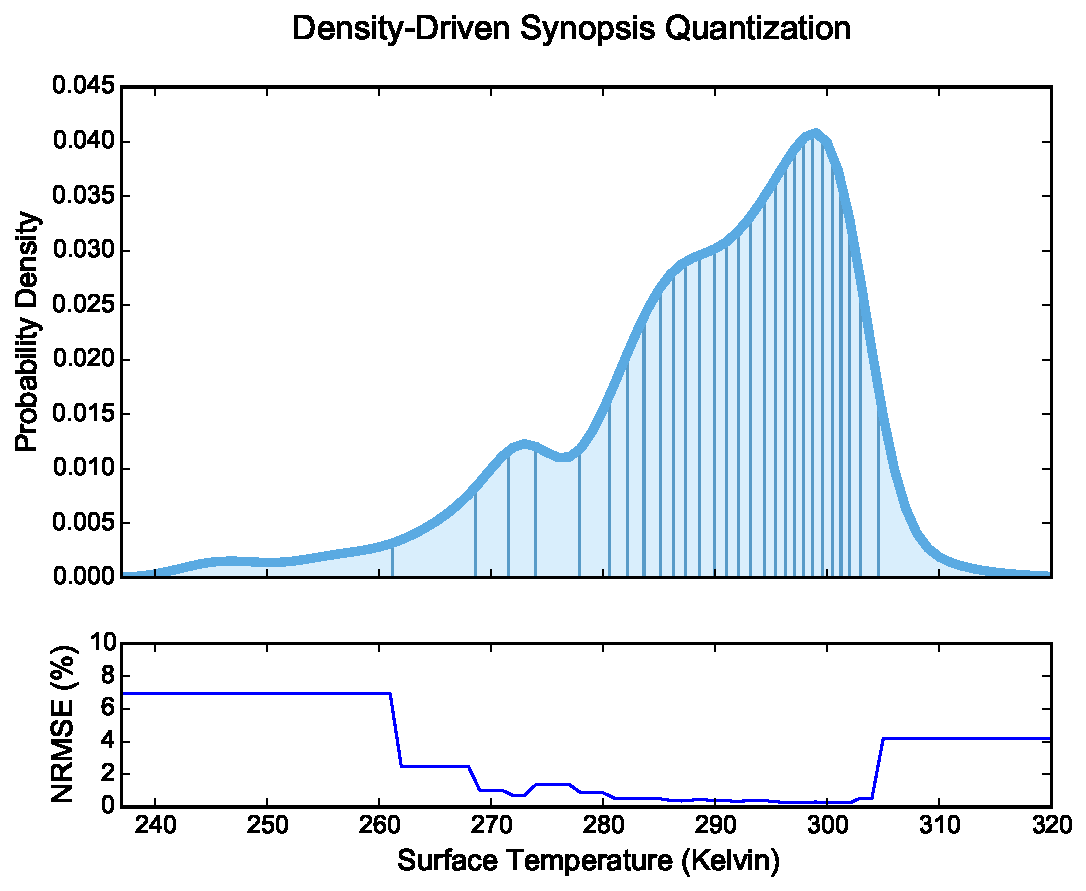
\includegraphics[width=3.5in]{figures/quantization.pdf}}
    \caption{A demonstration of the quantization process, with 29 vertex bins generated across the distribution of surface temperature values in our dataset. Each bin is indicated by a vertical line under the curve.}
    \label{fig:quantization}
\end{figure}

\begin{table}[h!]
    \renewcommand{\arraystretch}{1.3}
    \caption{Graph statistics (before/after quant)}
    \label{tbl:graph-stats}
    \begin{center}
        \begin{tabular}{|l|c|c|c|}
            \hline
            Configuration & Vertices & Edges & Leaves \\
            \hline
            A & & & \\
            \hline
            B & & & \\
            \hline
            C & & & \\
            \hline
        \end{tabular}
    \end{center}
\end{table}

\subsection{Temporal Dimensionality Reduction}
While our quantization approach enables Synopsis to retain large volumes of data in main memory, we also offer a temporal \emph{accuracy gradient} to ensure the most relevant data points are prioritized for high accuracy. This is achieved by iteratively removing features from the Synopsis hierarchy in the oldest subgraphs, eventually phasing out old records. A user-defined ``length of study'' (for instance, 12 months) informs the system when dimensionality reduction can begin. As data ages, this process results in the creation of temporal accuracy bands.

Selective temporal dimensionality reduction proceeds in a bottom-up fashion, starting from the leaf nodes. Given a set of relevant vertices, neighboring bins are merged uniformly across the feature space. As the bins are merged, their respective metadata is also merged, reducing memory consumption. Given two metadata instances, merging results in half the memory footprint. However, it is worth noting that this process is irreversible -- once metadata has been merged, it cannot be split at a later point in time. As time passes, entire feature planes are removed from the graph until a single metadata record is left for a particular temporal range. This allows users to still query the summary statistics and models for historical data, but at a lower level of accuracy.

\begin{table}[h!]
    \renewcommand{\arraystretch}{1.3}
    \caption{Graph statistics (after temp. reduction)}
    \label{tbl:graph-stats}
    \begin{center}
        \begin{tabular}{|l|c|c|c|}
            \hline
            Synopsis Age & Vertices & Edges & Leaves \\
            \hline
            1 month & & & \\
            \hline
            6 months & & & \\
            \hline
            12 months & & & \\
            \hline
        \end{tabular}
    \end{center}
\end{table}


